%----------------------------------------------------------------------------------------
%   PACKAGES AND THEMES
%----------------------------------------------------------------------------------------

\documentclass[aspectratio=169]{beamer}

\mode<presentation> {

% The Beamer class comes with a number of default slide themes
% which change the colors and layouts of slides. Below this is a list
% of all the themes, uncomment each in turn to see what they look like.

%\usetheme{default}
%\usetheme{AnnArbor}
%\usetheme{Antibes}
%\usetheme{Bergen}
%\usetheme{Berkeley}
%\usetheme{Berlin}
%\usetheme{Boadilla}
%\usetheme{CambridgeUS}
%\usetheme{Copenhagen}
%\usetheme{Darmstadt}
%%%%%%%\usetheme{Dresden}
%\usetheme{Frankfurt}
%\usetheme{Goettingen}
%\usetheme{Hannover}
%\usetheme{Ilmenau}
%\usetheme{JuanLesPins}
\usetheme{Luebeck}
%\usetheme{Madrid} 
%\usetheme{Malmoe}
%\usetheme{Marburg}
%\usetheme{Montpellier}
%\usetheme{PaloAlto}
%\usetheme{Pittsburgh}
%\usetheme{Rochester}
%\usetheme{Singapore}
%\usetheme{Szeged}
%\usetheme{Warsaw}

% As well as themes, the Beamer class has a number of color themes
% for any slide theme. Uncomment each of these in turn to see how it
% changes the colors of your current slide theme.

%\usecolortheme{albatross}
%%%%%\usecolortheme{beaver}
%\usecolortheme{beetle}
%\usecolortheme{crane}
%\usecolortheme{dolphin}
%\usecolortheme{dove}
%\usecolortheme{fly}
%\usecolortheme{lily}
%\usecolortheme{orchid}
%\usecolortheme{rose}
%\usecolortheme{seagull}
%\usecolortheme{seahorse}
%\usecolortheme{whale}
%\usecolortheme{wolverine}
\usecolortheme{default}

%\setbeamertemplate{footline} % To remove the footer line in all slides uncomment this line
%\setbeamertemplate{footline}[page number] % To replace the footer line in all slides with a simple slide count uncomment this line

%\setbeamertemplate{navigation symbols}{} % To remove the navigation symbols from the bottom of all slides uncomment this line
}


\addtobeamertemplate{navigation symbols}{}{%
    \usebeamerfont{footline}%
    \usebeamercolor[fg]{footline}%
    \hspace{1em}%
    \insertframenumber/\inserttotalframenumber
}



\usepackage{graphicx} % Allows including images
\usepackage{booktabs} % Allows the use of \toprule, \midrule and \bottomrule in tables
\usepackage[utf8]{inputenc}

\usepackage{ragged2e}
\usepackage{lmodern}
\usepackage{array}
\usepackage[normalem]{ulem}
\usepackage{microtype}

\usepackage{graphicx}
\graphicspath{ {images/} }

\setbeamerfont{footnote}{size=\tiny}

%----------------------------------------------------------------------------------------
%   TITLE PAGE
%----------------------------------------------------------------------------------------


\title[Protocolos de Experimentação]{Planejamento de Protocolos de Experimentação em Engenharia
de Software usando \textit{Business Process Model}} 
% The short title appears at the bottom of every slide, the full title is only on the title page

\author[Leandro Ungari Cayres]{Leandro Ungari Cayres \\Orientador: Prof. Dr. Rogério Eduardo Garcia} % Your name

\institute[UNESP] % Your institution as it will appear on the bottom of every slide, may be shorthand to save space
{
Universidade Estadual Paulista \\ % Your institution for the title page
\medskip
\textit{leandroungari@gmail.com} % Your email address
}
\date{22 de Janeiro de 2018} % Date, can be changed to a custom date

\begin{document}

\begin{frame}
\titlepage % Print the title page as the first slide
\end{frame}

%----------------------------------------------------------------------------------------
%   PRESENTATION SLIDES
%----------------------------------------------------------------------------------------
%\begin{frame}
%\frametitle{Visão Geral}
%\tableofcontents
%\end{frame}

\section{Introdução}

%==================
\begin{frame}
\frametitle{Problemática}
\justifying

A execução de experimentos controlados envolve o controle de parâmetros específicos para mensurar a influência desses em variáveis dependentes, assim como, a definição de um protocolo de execução.

\end{frame}

%==================
\begin{frame}
\frametitle{Problemática}
\justifying

Embora sugerido pelo Processo de Experimentação, o protocolo não fica explícito no pacote de laboratório e, consequentemente, não é visível ao experimentador e ao replicador. Desse modo, esta ausência de informação contribui para dificuldades na realização de replicação de experimentos.

\end{frame}

%==================

\begin{frame}
\frametitle{Objetivos Gerais}
\justifying

\begin{itemize}
\item Prover uma interface capaz de representar visualmente o protocolo de um experimento, através da notação BPM:
\end{itemize}
\end{frame}

%==================
\begin{frame}
\frametitle{Objetivos Gerais}
\justifying

\begin{itemize}
\item Prover uma interface capaz de representar visualmente o protocolo de um experimento, através da notação BPM:
\\~\\
\begin{enumerate}
\item Possibilitar ao experimentador a possibilidade de planejamento e construção do protocolo de experimentação.
\end{enumerate}
\end{itemize}
\end{frame}

%==================
\begin{frame}
\frametitle{Objetivos Gerais}
\justifying

\begin{itemize}
\item Prover uma interface capaz de representar visualmente o protocolo de um experimento, através da notação BPM:
\\~\\
\begin{enumerate}
\item Possibilitar ao experimentador a possibilidade de planejamento e construção do protocolo de experimentação.
\item Viabilizar a visualização do protocolo de experimentação contido em um pacote de laboratório.
\end{enumerate}
\end{itemize}
\end{frame}

\begin{frame}
\frametitle{Objetivos Específicos}
\justifying
\begin{itemize}
\item Aplicação de modificações na camada de apresentação da ferramenta \textit{OntoExpTool}, incorporando o modelo gráfico a esta, e consequentemente, as alterações necessárias na camada de controle.
\end{itemize}

\end{frame}

\begin{frame}
\frametitle{Objetivos Específicos}
\justifying

\begin{itemize}
\item Aplicação de modificações na camada de apresentação da ferramenta \textit{OntoExpTool}, incorporando o modelo gráfico a esta, e consequentemente, as alterações necessárias na camada de controle.
\\~\\
\item Construção de um sistema de software que possibilite a concepção e troca de pacotes de laboratório, para a condução de experimentos controlados.

\end{itemize}
\end{frame}

\section{Processo de Experimentação}

\begin{frame}
\frametitle{Experimentos Controlados}
\justifying


\begin{itemize}
\item A condução de experimentos controlados tem sua execução manipulada de forma direta e sistemática, a fim de se ter controle sob todos os elementos que o compõem. 
\item Objetos representativos são selecionados, os quais compõem as variáveis analisadas no estudo. 
\item Tem execução em ambientes controlados.
\end{itemize}

\end{frame}

\begin{frame}
\frametitle{Processo de Experimentação}
\justifying

Desse modo, a execução de um estudo requer uma sequência de atividades estabelecidas previamente, pelas quais seja possível conduzir um processo experimental de modo \underline{preciso} e \underline{sistemático}.


\end{frame}

\begin{frame}
\frametitle{Processo de Experimentação}
\justifying

\begin{center}
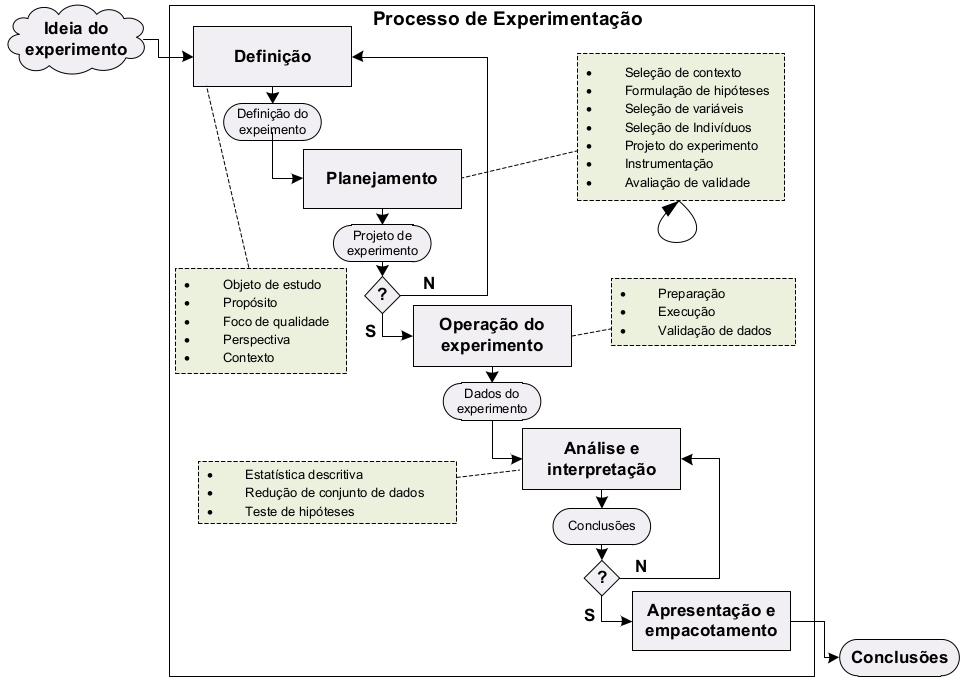
\includegraphics[width=0.5\textwidth]{experimento.png}
\end{center}


\end{frame}




\section{Modelo de Processo de Negócio}

\begin{frame}
\frametitle{Modelo de Processo de Negócio}
\justifying

Um processo de negócio é descrito por um ou mais procedimentos que, de modo conjunto, focam a realização de um objetivo de negócio. A execução de um processo de negócio possui condições muito bem definidas de início e término, e pode combinar procedimentos automáticos e/ou manuais.


\end{frame}

\begin{frame}
\frametitle{\textit{Business Process Modeling and Notation}}
\justifying

\begin{center}
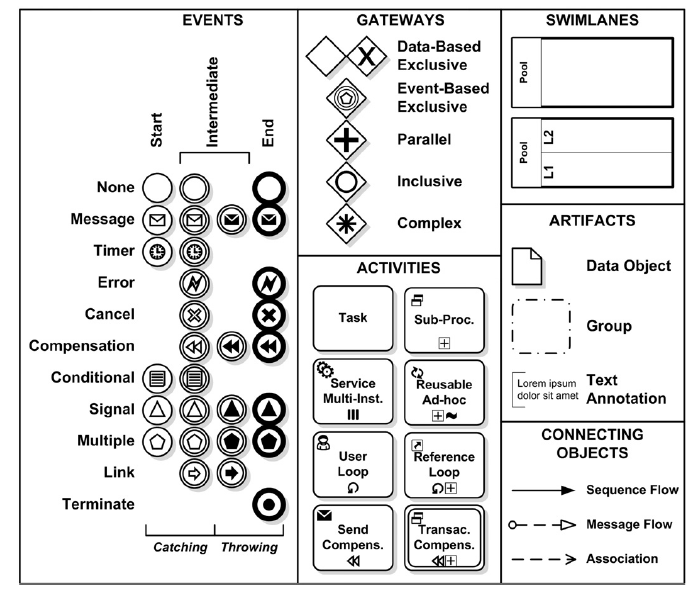
\includegraphics[width=0.45\textwidth]{elementos.png}
\end{center}


\end{frame}

\begin{frame}
\frametitle{Modelo de Processo de Negócio}
\justifying

\begin{center}
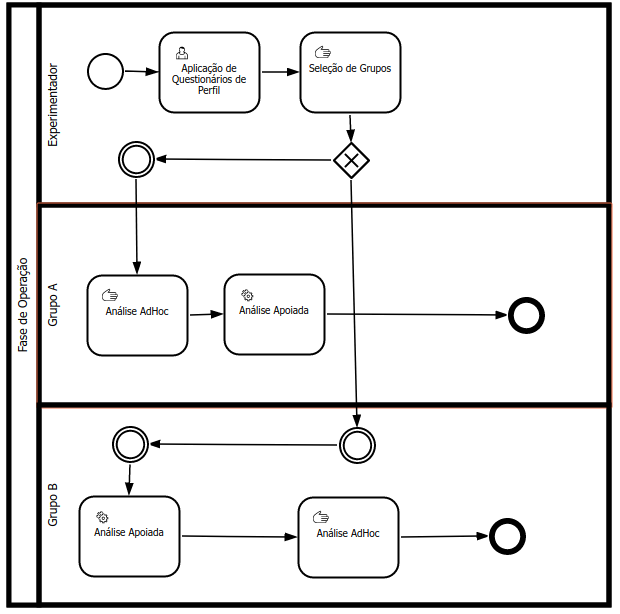
\includegraphics[width=0.4\textwidth]{protocolo.png}
\end{center}


\end{frame}

\begin{frame}
\frametitle{Modelo de Processo de Negócio}
\justifying

\begin{center}
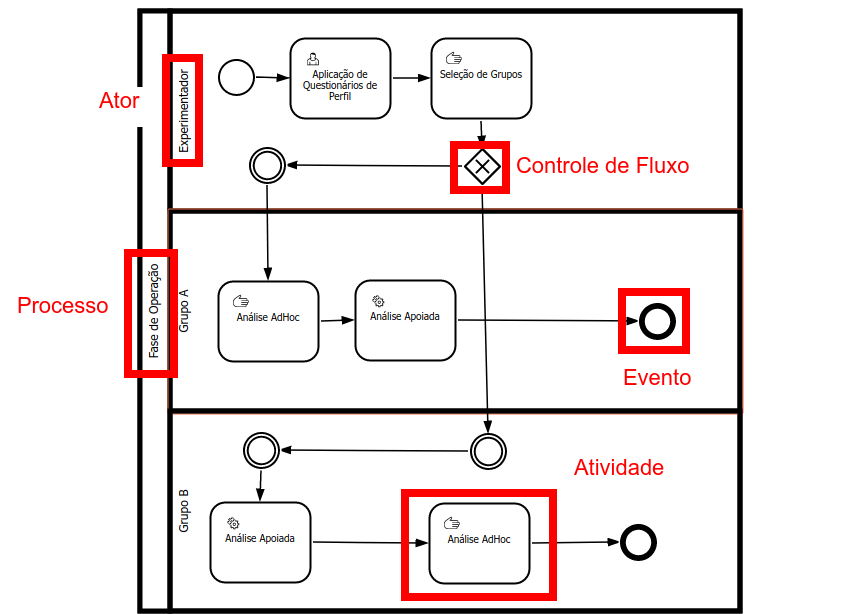
\includegraphics[width=0.55\textwidth]{explicado.png}
\end{center}


\end{frame}

\section{Pacote de Laboratório}

\begin{frame}
\frametitle{Pacote de Laboratório}
\justifying

Diversas pesquisas, técnicas e ferramentas têm sido desenvolvidos para avaliar modelos ou otimizar soluções. Porém, tais recursos ou informações isoladas não formam um corpo de conhecimento consistente, então tornando necessário compartilhá-los entre os grupos de pesquisa por meio do uso de
pacotes de laboratório.

\end{frame}

\begin{frame}
\frametitle{Pacote de Laboratório}
\justifying

\begin{center}
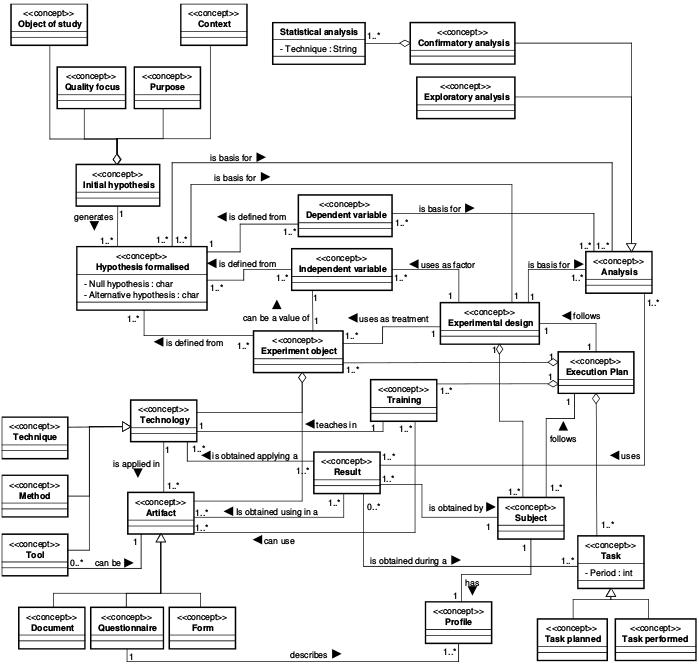
\includegraphics[width=0.4\textwidth]{onto.png}
\end{center}

\end{frame}


\begin{frame}
\frametitle{Implementação}
\justifying

\begin{columns}
\begin{column}{0.5\textwidth}

Camada de Persistência do Experimento: modelo de classes baseado na ontologia \textit{ExperOntology}.\\
\begin{itemize}
\item Quantidade de classes: 30.
\end{itemize}
   
\end{column}
\begin{column}{0.5\textwidth} 
    \begin{center}
     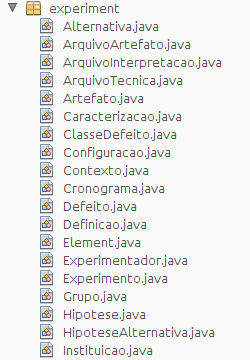
\includegraphics[width=0.5\textwidth]{pacote-experimento.png}
     \end{center}
\end{column}
\end{columns}

\end{frame}

%==================
\begin{frame}
\frametitle{Implementação}
\justifying

\begin{center}
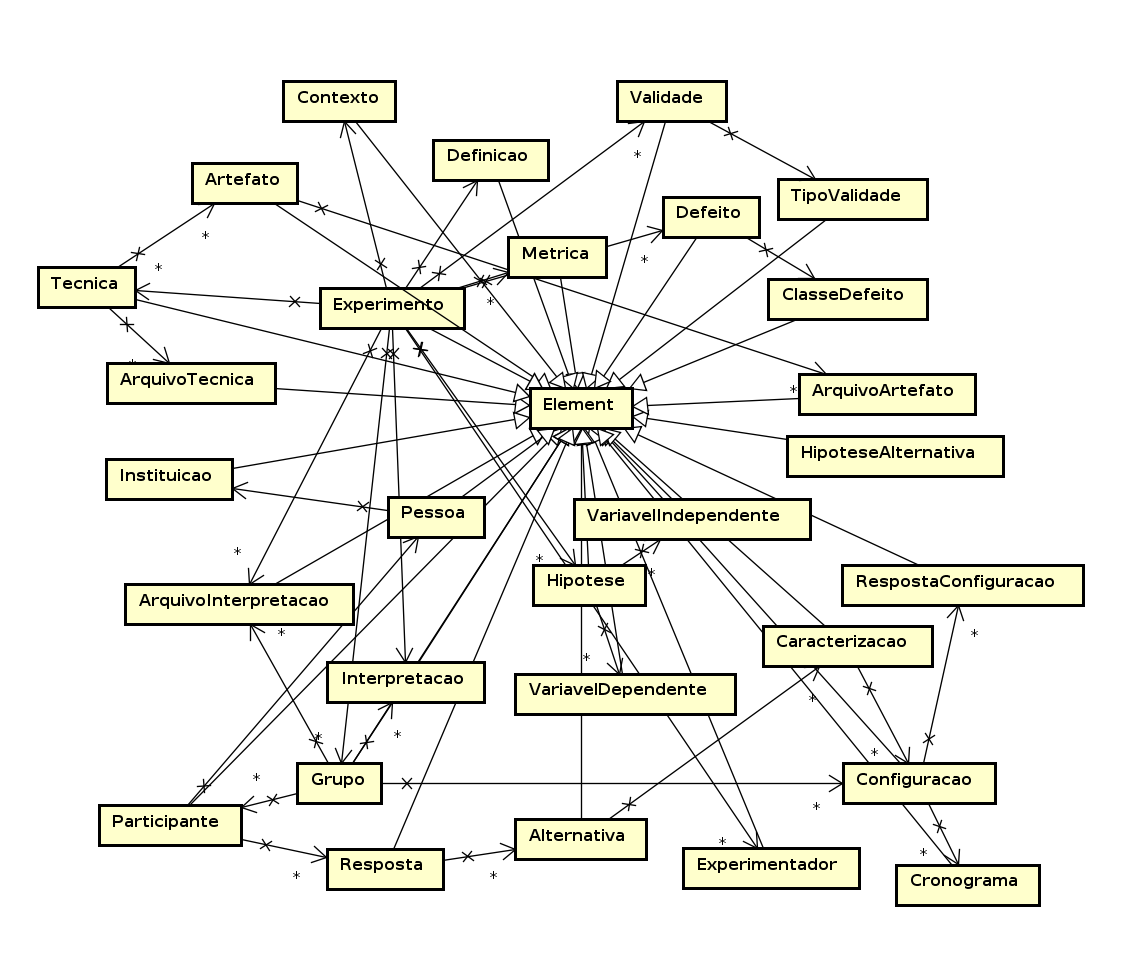
\includegraphics[width=0.5\textwidth]{diagrama-classes-experimento.png}
\end{center}

\end{frame}

%==================
\begin{frame}
\frametitle{Implementação}
\justifying

\begin{columns}
\begin{column}{0.5\textwidth}

Camada de Persistência da Notação BPM: modelo de classes dos elementos gráficos que compõem a notação de modelo de processo de negócio.\\
\begin{itemize}
\item Quantidade de pacotes: 10.
\item Quantidade de classes: 86.
\end{itemize}
   
\end{column}
\begin{column}{0.5\textwidth} 
    \begin{center}
     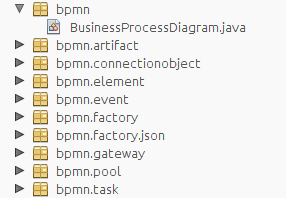
\includegraphics[width=0.7\textwidth]{pacote-bpmn.png}
     \end{center}
\end{column}
\end{columns}

\end{frame}

%==================
\begin{frame}
\frametitle{Implementação}
\justifying

\begin{center}
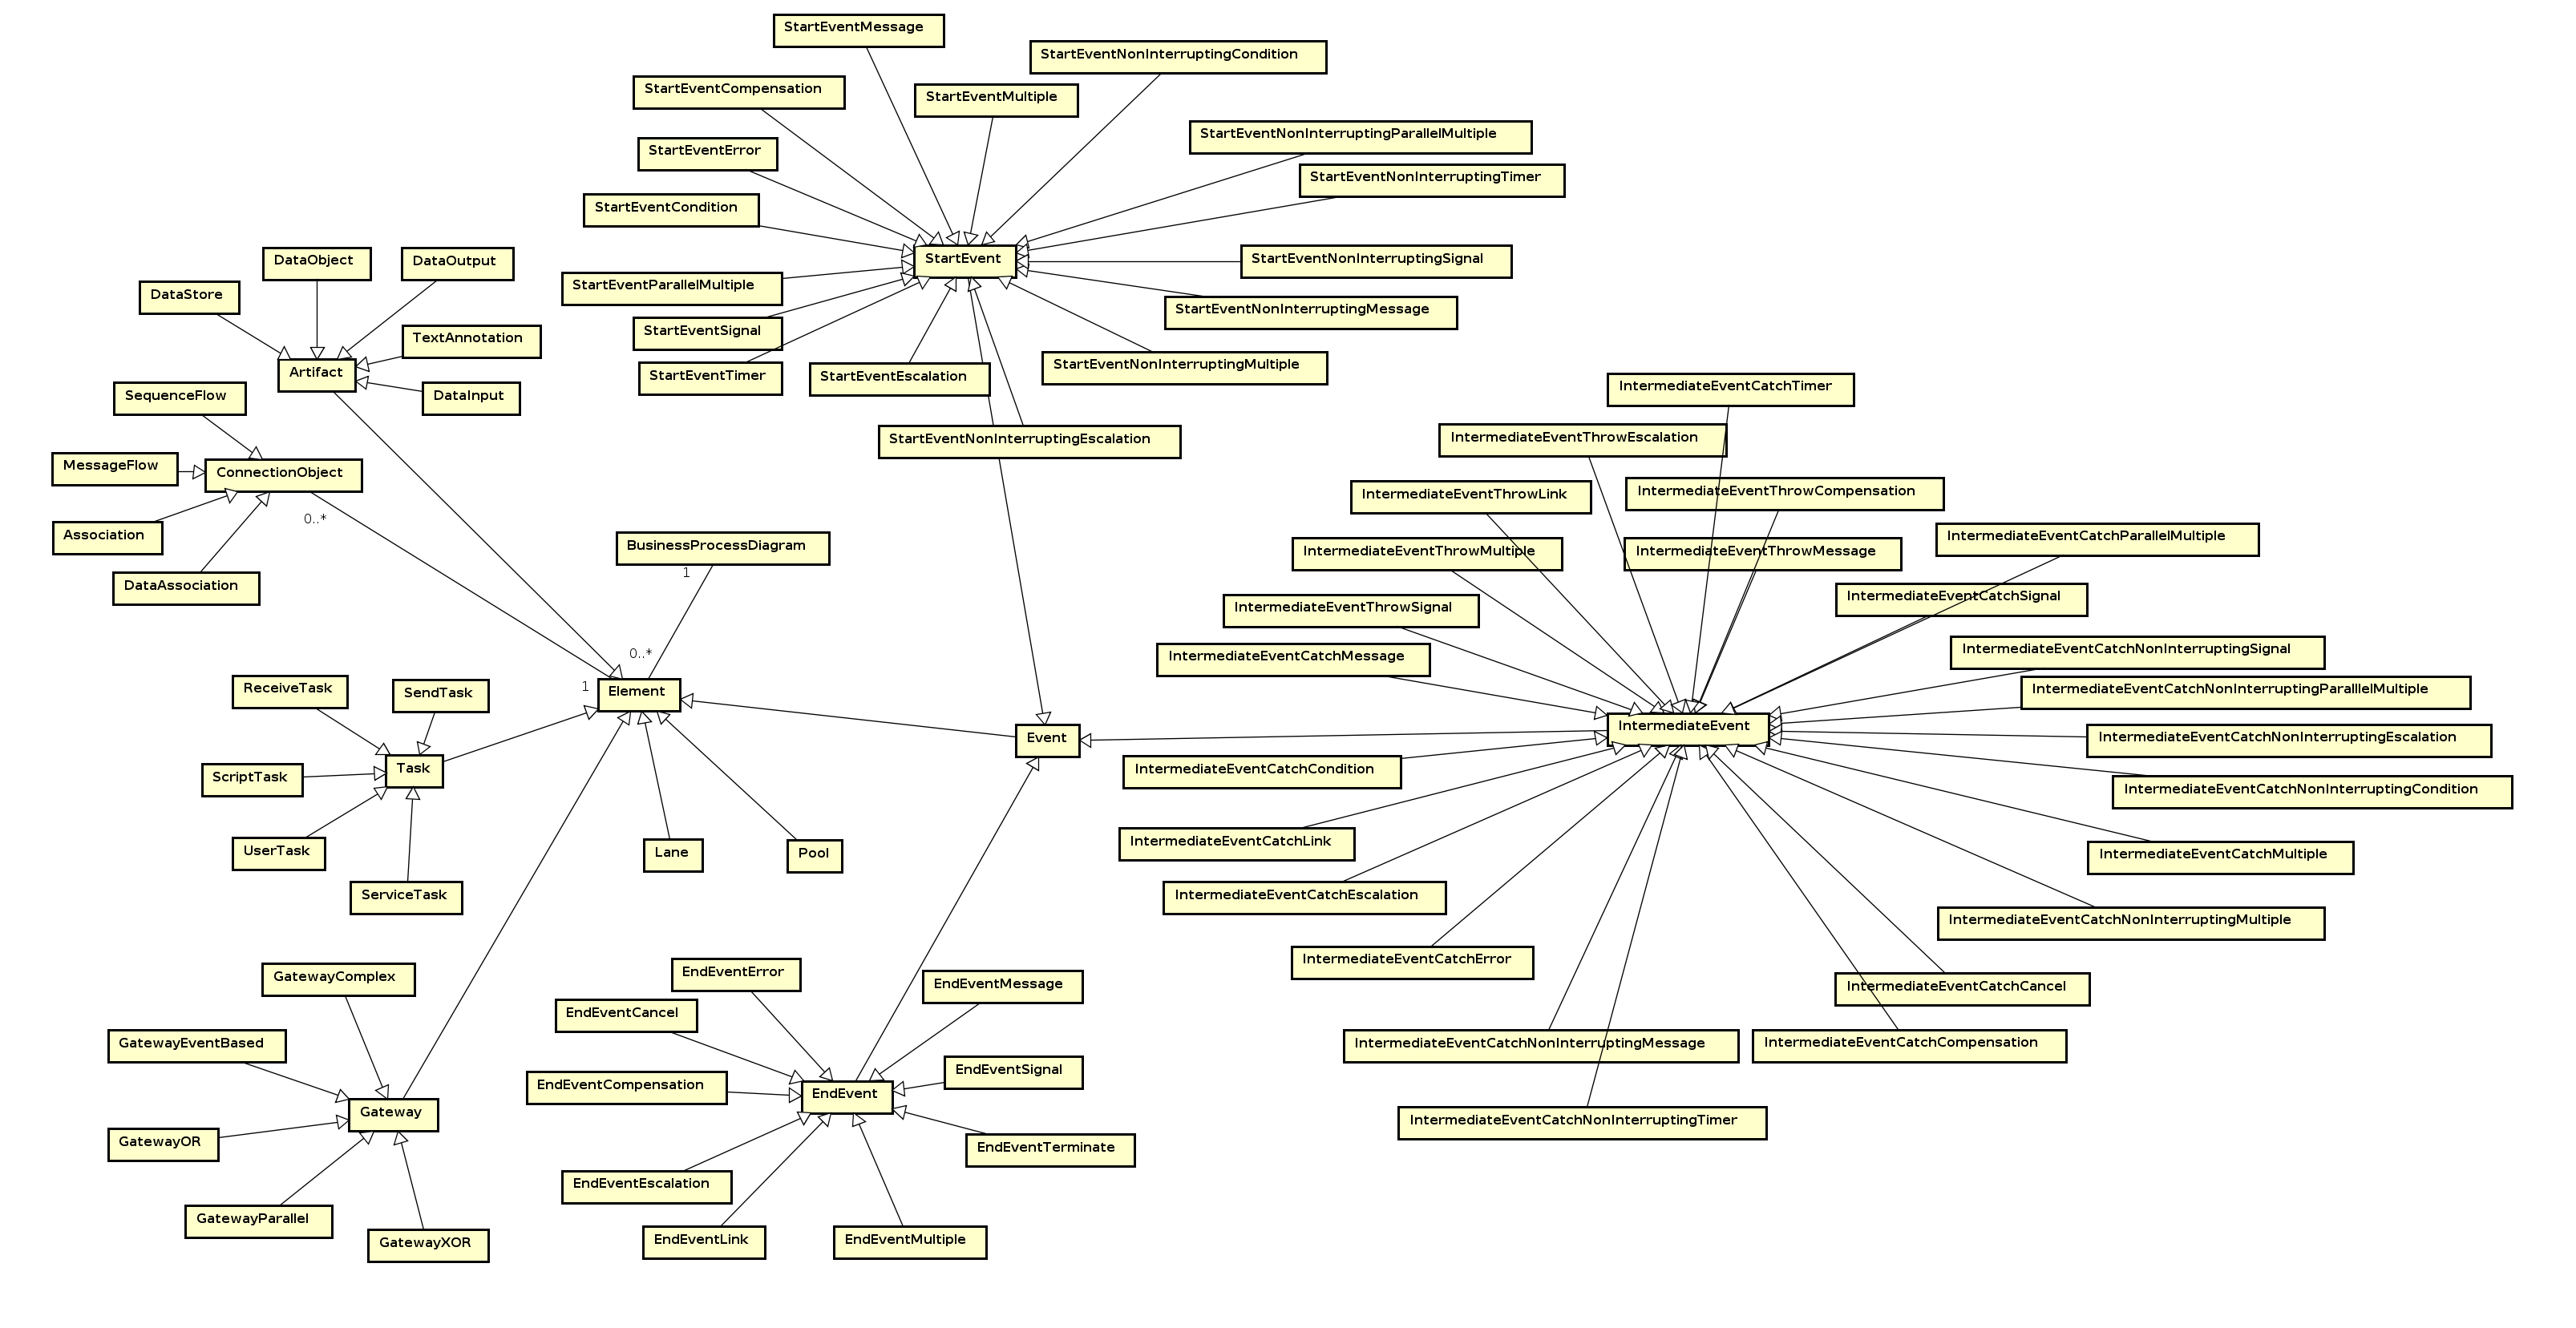
\includegraphics[width=.85\textwidth]{diagrama-classes-bpmn.png}
\end{center}

\end{frame}

\begin{frame}
\frametitle{Ferramenta}
\justifying

As tecnologias utilizadas foram: 
\begin{itemize}
\item HTML 5, CSS 3 para a construção do layout da ferramenta.
\item JavaScript e as bibliotecas JQuery e D3.js para a interação e funcionalidades da ferramenta.
\item Biblioteca XStream para a persistência do pacote de laboratório.
\item Java Server Pages e GlassFish Server para a camada de controle do servidor.
\end{itemize}

\end{frame}


\begin{frame}
\frametitle{Atividades Futuras}
\justifying

\begin{itemize}
\item Instanciação de pacotes laboratório de outros experimentos previamente conduzidos. 
\item Avaliação por parte do experimentador de cada experimento.
\item Condução de experimentos em relação à interface quanto a usabilidade e funcionalidade.
\end{itemize}


\end{frame}

\begin{frame}
\frametitle{Exemplo}
\justifying

\begin{itemize}
\item Experimento Controlado
\item Avaliação da ferramenta de visualização de software \textit{SoftVisOAH} como apoio à depuração de programas: um experimento controlado.
\item Experimentador: Álvaro Ferraz d’Arce.
\item Ano: 2012.
\end{itemize}


\end{frame}



%\begin{columns}
%\begin{column}{0.5\textwidth}
   
   
%\end{column}
%\begin{column}{0.5\textwidth} 
%    \begin{center}
%     \includegraphics[width=0.5\textwidth]{image1.jpg}
%     \end{center}
%\end{column}
%\end{columns}


%----------------------------------------------------------------------------------------


\end{document}


              
            